\section{System Architecture}

A general concern when designing large systems is the accidental
complexity\cite[p.~8-9]{holt2004uml} one may create by poor design choices early
on. Many solutions designed to reduce accidental complexity are based around
software systems, and sacrifices performance in both the time domain and in the
space domain\cite{moseley2006out}. While these solutions may be applicable
within hardware systems where these kinds of performance degradations are not a
problem, it is unacceptable in systems where one or multiple of the system
requirements are a performance increase in one or both of these domains. As one
of our main requirements is focus on performance, we have to accept a certain
level of inherent complexity.
\begin{figure}[h]
  \centering
  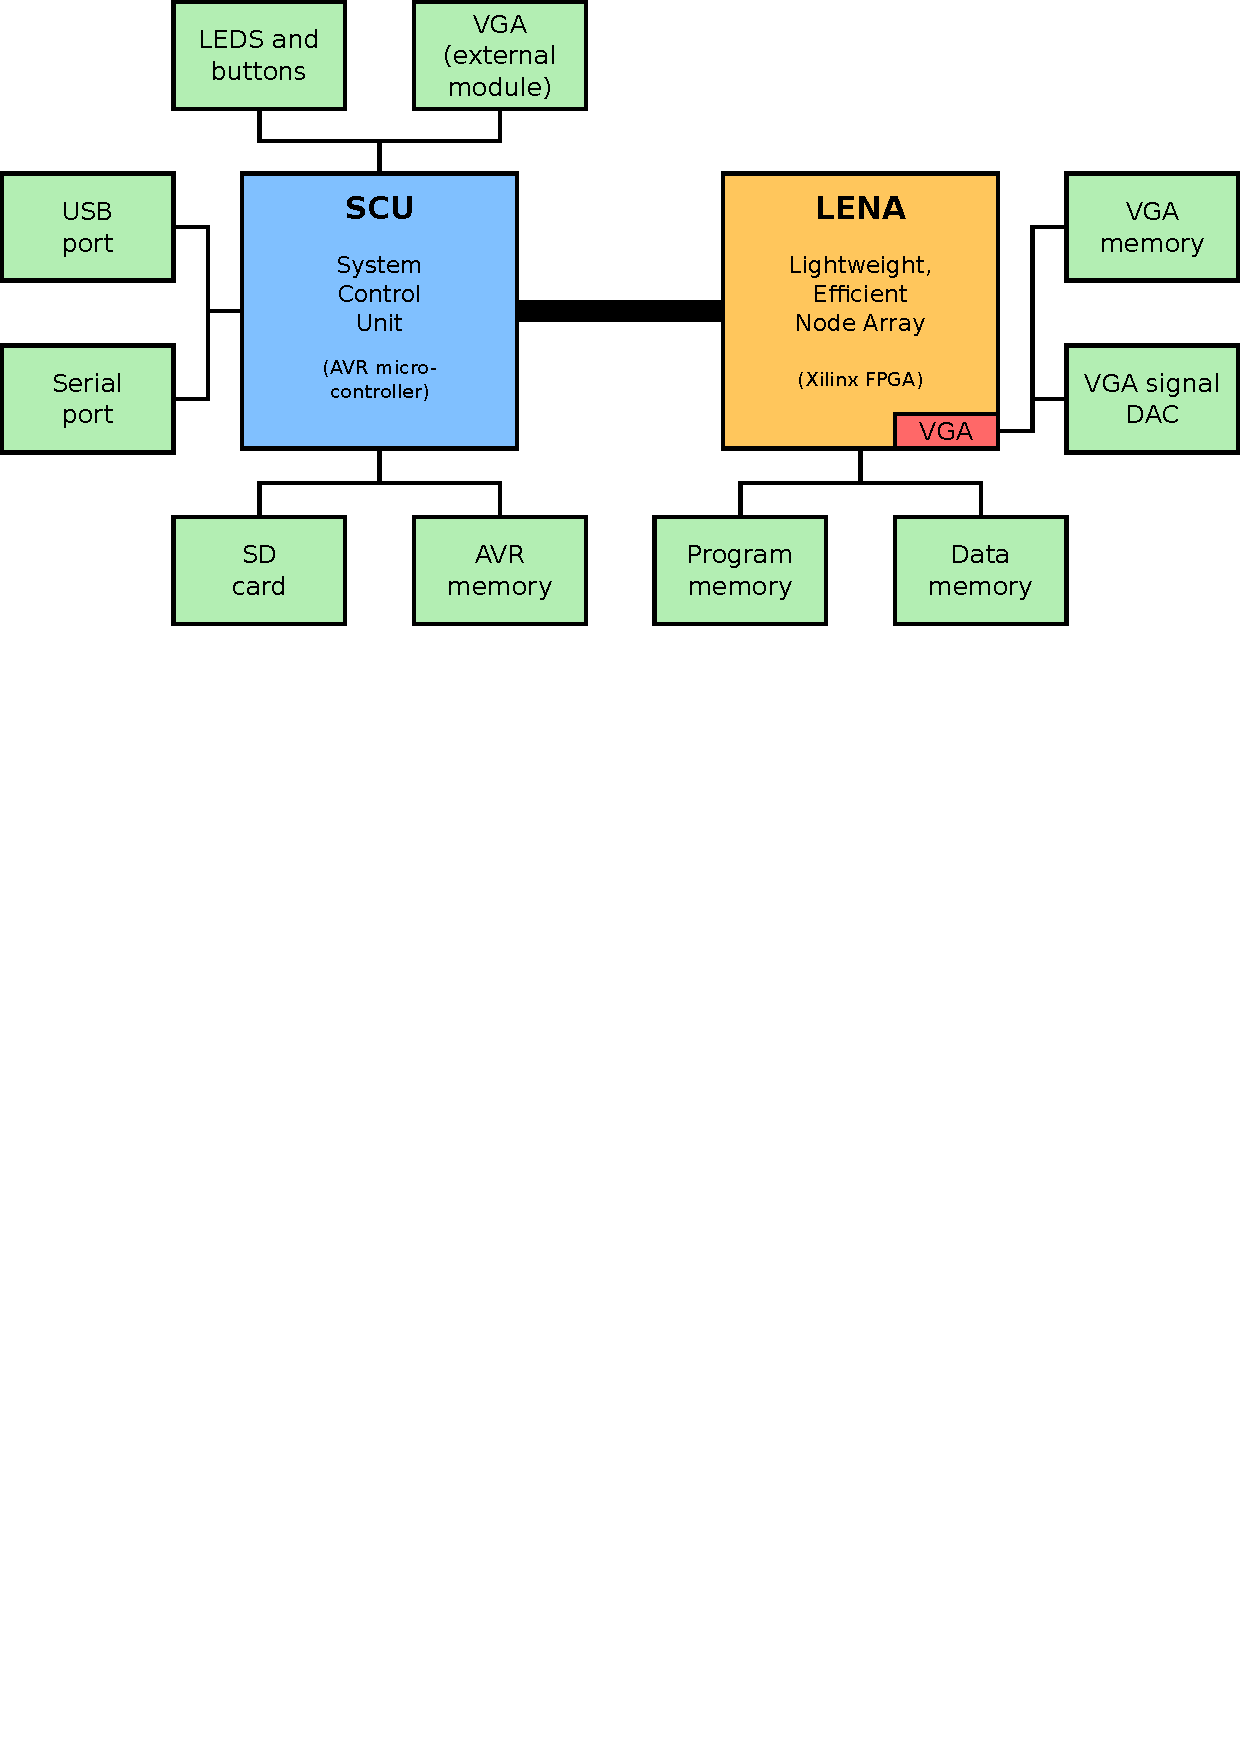
\includegraphics[width=\linewidth,clip,trim=0 18cm 0 0]
                  {fig/sys-over/arch-fig.pdf}
  \caption{System Architecture}
  \label{fig:sys-over-arch-fig}
\end{figure}


To remedy the complexity which comes from our requirements, we focused on making
it possible to isolate errors and make it possible to test the individual
components as fast as possible: The \ac{LENA} architecture was tested through
\ac{VHDL} test benches, the \ac{VGA} component in the \ac{LENA} architecture was
tested with \acp{LED} and buttons on the board, and the AVR part of the
\ac{LENA} system was tested through the \ac{VGA} port on the board. By doing
this, we can assume that errors occurring when connecting different components is
due to errors in the protocol implementation(s).

Figure \ref{fig:sys-over-arch-fig} shows our resulting architecture. Buttons and
\acp{LED} made it easy to confirm that the \ac{VGA} operates properly for simple
programs. A \ac{VGA} connector made it possible to quickly test and debug the
\ac{VGA} implementation on the \ac{LENA} architecture. We also included a
\ac{VGA} connector connected to the AVR, in case the \ac{LENA} architecture
should fail to implement its \ac{VGA} module.

To be able to process data, we need an \ac{I/O} device which serves the machine
with data it should process. To ensure that we would have at least one
functional \ac{I/O} component,\CHECK{Sounds okay now?} we included both a serial
port, a \ac{USB} port and a \ac{SD} card reader on the \ac{PCB}.

The \ac{LENA} architecture has three different memory components: One for the
\ac{VGA} component, one for instructions and one for data. The main reason for
this is that image processing systems in general need a lot of memory. The
\ac{VGA} module needs to constantly send out an image to the \ac{VGA} port, so
it needs to keep the old image in memory. The \ac{LENA} architecture should have
one image in memory which it can send to the \ac{SIMD} nodes, and one image
which is currently read from the \ac{SCU} to memory. In addition, one would have
to read data instructions as well. All these different parts require relatively
much memory, and they are all frequently accessed. Therefore, it would be
favorable to have them as separate components so that memory access can be
parallelised.
